% =============================================================================
%  A Crash Course in Graph Databases with neo4j  —  StatBytes, Nov 4 2026
%  Joshua Ingram, CMU Statistics & Data Science
%
%  Build:  latexmk -pdf statbytes_neo4j.tex     (figures in ../demo/figures)
%  Edit:   search for "% ===== SLIDE" to jump to a slide; numbers match PDF pages.
% =============================================================================
\documentclass[aspectratio=169, 10pt]{beamer}

\usepackage[T1]{fontenc}
\usepackage[utf8]{inputenc}
\usepackage{lmodern}
\usepackage{amsmath}
\usepackage{tikz}
\usetikzlibrary{positioning, arrows.meta, calc, matrix}
\usepackage{tcolorbox}
\tcbuselibrary{skins, listings}
\usepackage{listings}
\usepackage{booktabs}
\usepackage{graphicx}
\usepackage{xcolor}
\usepackage{hyperref}

% ------------------------------------------------------------------ palette
\definecolor{forest}{HTML}{1F4D32}     % primary: dark forest green
\definecolor{moss}{HTML}{3C7A54}       % lighter green for rules/accents
\definecolor{burgundy}{HTML}{7A1F2B}   % secondary / highlight
\definecolor{ink}{HTML}{1E2A24}
\definecolor{muted}{HTML}{66736C}
\definecolor{codebg}{HTML}{1B2B22}
\definecolor{codefg}{HTML}{E9EFEA}
\definecolor{codekw}{HTML}{9CD3B4}
\definecolor{codestr}{HTML}{E8B86D}
\definecolor{codecom}{HTML}{98A89F}
% tinted boxes (border / fill)
\definecolor{bgreen}{HTML}{3C7A54}   \definecolor{fgreen}{HTML}{EEF5F0}
\definecolor{bburg}{HTML}{7A1F2B}    \definecolor{fburg}{HTML}{F8ECEE}
\definecolor{bgold}{HTML}{B07D2B}    \definecolor{fgold}{HTML}{FBF4E6}
\definecolor{bslate}{HTML}{4A6B8A}   \definecolor{fslate}{HTML}{EDF2F7}
\definecolor{bgray}{HTML}{8A9A91}    \definecolor{fgray}{HTML}{F2F4F3}

% ------------------------------------------------------------------ beamer theme
\usetheme{default}
\usefonttheme{professionalfonts}
\setbeamertemplate{navigation symbols}{}
\setbeamercolor{normal text}{fg=ink}
\setbeamercolor{structure}{fg=forest}
\setbeamercolor{frametitle}{fg=forest}
\setbeamercolor{itemize item}{fg=burgundy}
\setbeamercolor{itemize subitem}{fg=burgundy}
\setbeamercolor{enumerate item}{fg=burgundy}
\setbeamertemplate{itemize item}{\textbullet}
\setbeamertemplate{itemize subitem}{--}
\setbeamerfont{frametitle}{size=\large, series=\bfseries}
\setbeamertemplate{frametitle}{%
  \vspace{0.25cm}\insertframetitle\par\vspace{-0.12cm}%
  {\color{moss}\rule{\textwidth}{0.8pt}}\vspace{-0.1cm}%
}
\setbeamertemplate{footline}{%
  \hspace{0.5cm}{\scriptsize\color{muted}Graph Databases with neo4j}\hfill
  {\scriptsize\color{muted}\insertframenumber\,/\,\inserttotalframenumber}\hspace{0.4cm}\vspace{0.2cm}%
}
\setlength{\leftmargini}{1.1em}
\setbeamersize{text margin left=0.7cm, text margin right=0.7cm}
\setbeamertemplate{itemize/enumerate body begin}{\setlength{\itemsep}{2pt}}

% ------------------------------------------------------------------ code style
\lstdefinelanguage{Cypher}{
  morekeywords={MATCH, OPTIONAL, WHERE, RETURN, WITH, CREATE, MERGE, SET, DELETE, DETACH, REMOVE,
    ORDER, BY, LIMIT, SKIP, AS, AND, OR, NOT, DISTINCT, CALL, YIELD, LOAD, CSV, HEADERS, FROM,
    UNWIND, UNION, ALL, CONSTRAINT, INDEX, IF, EXISTS, FOR, REQUIRE, IS, UNIQUE, ON, OPTIONS, VECTOR, IN},
  sensitive=false, morecomment=[l]{//}, morestring=[b]', morestring=[b]"
}
\lstdefinelanguage{json}{morestring=[b]", sensitive=false}
\lstdefinelanguage{yaml}{morekeywords={services,image,ports,environment,volumes}, morecomment=[l]{\#}, morestring=[b]', morestring=[b]", sensitive=true}
\lstset{
  basicstyle=\ttfamily\scriptsize\color{codefg},
  keywordstyle=\color{codekw}\bfseries, stringstyle=\color{codestr}, commentstyle=\color{codecom}\itshape,
  showstringspaces=false, breaklines=true, columns=fullflexible, keepspaces=true, tabsize=2,
}
\newtcblisting{code}[1][Cypher]{
  enhanced, listing only, colback=codebg, colframe=codebg, arc=2pt, boxrule=0pt,
  left=5pt, right=5pt, top=3pt, bottom=3pt, listing options={language=#1},
}
\newtcblisting{codesmall}[1][Cypher]{
  enhanced, listing only, colback=codebg, colframe=codebg, arc=2pt, boxrule=0pt,
  left=4pt, right=4pt, top=2pt, bottom=2pt, listing options={language=#1, basicstyle=\ttfamily\tiny\color{codefg}},
}
\newcommand{\chip}[1]{\colorbox{codebg}{\color{codefg}\ttfamily\scriptsize #1}}

% ------------------------------------------------------------------ tinted box
% \begin{tbox}[Title]{bordercolor}{fillcolor} ... \end{tbox}
\newtcolorbox{tbox}[3][]{enhanced, colback=#3, colframe=#2, arc=4pt, boxrule=1pt,
  left=5pt, right=5pt, top=4pt, bottom=4pt, boxsep=0pt,
  title={#1}, detach title, coltitle=#2, fonttitle=\small\bfseries,
  before upper={\tcbtitle\par\vspace{2pt}}, fontupper=\small\raggedright}
\newcommand{\kicker}[1]{{\color{muted}\small #1}}

% ------------------------------------------------------------------ dark slides
\newcommand{\partslide}[2]{% number, title
  {\setbeamercolor{background canvas}{bg=forest}
   \begin{frame}[plain]
     \begin{tikzpicture}[remember picture, overlay]
       \fill[burgundy] (current page.west) ++(0,-0.4) rectangle ++(0.18,1.9);
       \node[anchor=east, text=forest!70!white, font=\fontsize{120}{120}\selectfont\bfseries, opacity=0.3]
         at ($(current page.east)+(-0.3,0.1)$) {#1};
       \draw[burgundy, line width=0.6pt] ($(current page.south west)+(0,0.35)$) -- ($(current page.south east)+(0,0.35)$);
       \node[anchor=west, align=left, text=white] at ($(current page.west)+(0.7,0.35)$) {%
         {\ttfamily\footnotesize\color{burgundy!40!white}PART #1}\\[2pt]
         {\LARGE\bfseries #2}\\[-1pt]
         {\color{white!60!forest}\rule{5.5cm}{0.5pt}}};
     \end{tikzpicture}
   \end{frame}}}

\title{A Crash Course in Graph Databases with neo4j}
\author{Joshua D. Ingram}
\date{November 4, 2026}

\begin{document}

% ===== SLIDE 1: title =========================================================
{\setbeamercolor{background canvas}{bg=forest}
\begin{frame}[plain]
  \begin{tikzpicture}[remember picture, overlay]
    \fill[burgundy] (current page.west) ++(0,-0.2) rectangle ++(0.18,2.2);
    \node[anchor=west, align=left, text=white] at ($(current page.west)+(0.7,0.45)$) {%
      {\Huge\bfseries A Crash Course in}\\[2pt]
      {\Huge\bfseries Graph Databases with neo4j}\\[26pt]
      {\bfseries Joshua D. Ingram}\\[2pt]
      {\small Department of Statistics \& Data Science, Carnegie Mellon University}\\[2pt]
      {\small StatBytes, November 4, 2026}};
    \begin{scope}[shift={($(current page.east)+(-2.2,2.4)$)}, scale=0.75, every node/.style={circle, inner sep=0pt}]
      \node[fill=burgundy!80!white, minimum size=9pt] (a) at (0,0) {};
      \node[fill=white!70!forest, minimum size=7pt] (b) at (1.1,0.8) {};
      \node[fill=white!70!forest, minimum size=7pt] (c) at (1.3,-0.7) {};
      \node[fill=white!70!forest, minimum size=5pt] (d) at (2.2,0.1) {};
      \node[fill=white!70!forest, minimum size=5pt] (e) at (-0.9,0.9) {};
      \node[fill=white!70!forest, minimum size=5pt] (f) at (-1.0,-0.9) {};
      \node[fill=white!70!forest, minimum size=5pt] (g) at (2.3,1.2) {};
      \draw[white!55!forest, line width=1pt] (a)--(b) (a)--(c) (b)--(d) (c)--(d) (a)--(e) (a)--(f) (b)--(g) (d)--(g) (e)--(f);
    \end{scope}
  \end{tikzpicture}
\end{frame}}

% ===== SLIDE 2: overview ======================================================
\begin{frame}[fragile]{Overview}
  \vspace{0.3cm}
  \begin{columns}[T]
    \column{0.24\textwidth}
      \begin{tbox}[1 \ Overview of graphs and databases]{bgreen}{fgreen}
        What is a graph? Where does graph data show up? What are graph databases?
      \end{tbox}
    \column{0.24\textwidth}
      \begin{tbox}[2 \ Database setup and Cypher queries]{bslate}{fslate}
        Setting up a neo4j database, importing data, writing Cypher queries, Python usage, and system workflows
      \end{tbox}
    \column{0.24\textwidth}
      \begin{tbox}[3 \ Graph Data Science library]{bgold}{fgold}
        Introduction to the GDS library, graph projections, and centrality measures
      \end{tbox}
    \column{0.24\textwidth}
      \begin{tbox}[4 \ Knowledge graphs and RAG]{bburg}{fburg}
        Knowledge graphs, retrieval-augmented generation, GraphRAG, and neo4j's AI tools
      \end{tbox}
  \end{columns}
  \vspace{0.6cm}
  \centering
  Example data: a mock regional \textbf{power grid} (140 substations, 322 lines, 25 generators, 60 loads).
\end{frame}

% ===== PART 1 =================================================================
\partslide{01}{Graph data and graph databases}

% ===== SLIDE 4: what is a graph ===============================================
\begin{frame}[fragile]{What is a graph?}
  \vspace{0.1cm}
  A graph $G=(V,E)$ is a set of \textbf{nodes} $V$ and a set of \textbf{edges} $E$ between pairs of nodes. Nodes and edges can carry attributes.
  \vspace{0.2cm}
  \begin{columns}[T]
    \column{0.5\textwidth}
      \centering {\small\bfseries Undirected} --- an edge is a pair $\{i,j\}$\\[6pt]
      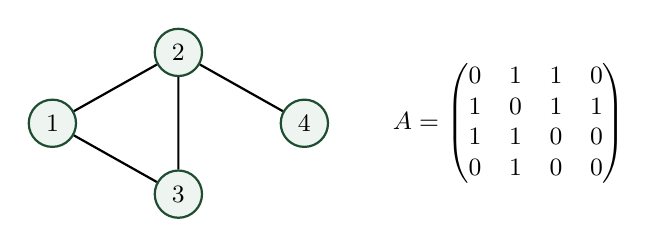
\begin{tikzpicture}[every node/.style={font=\small}, nd/.style={circle, draw=forest, fill=fgreen, thick, minimum size=0.6cm}]
        \node[nd] (1) at (0,0) {1};
        \node[nd] (2) at (1.6,0.9) {2};
        \node[nd] (3) at (1.6,-0.9) {3};
        \node[nd] (4) at (3.2,0) {4};
        \draw[thick] (1)--(2) (1)--(3) (2)--(3) (2)--(4);
        \node[anchor=west] at (4.2,0) {$A=\begin{pmatrix}0&1&1&0\\1&0&1&1\\1&1&0&0\\0&1&0&0\end{pmatrix}$};
      \end{tikzpicture}\\[4pt]
      \kicker{Adjacency matrix $A$: $A_{ij}=1$ if $i$ and $j$ are joined. Symmetric. Row sums are degrees.}
    \column{0.5\textwidth}
      \centering {\small\bfseries Directed} --- an edge is an ordered pair $(i,j)$\\[6pt]
      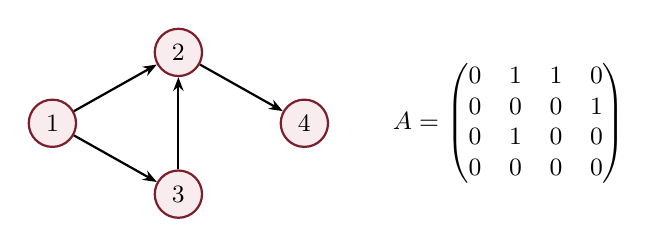
\begin{tikzpicture}[every node/.style={font=\small}, nd/.style={circle, draw=burgundy, fill=fburg, thick, minimum size=0.6cm}, >={Stealth[length=5pt]}]
        \node[nd] (1) at (0,0) {1};
        \node[nd] (2) at (1.6,0.9) {2};
        \node[nd] (3) at (1.6,-0.9) {3};
        \node[nd] (4) at (3.2,0) {4};
        \draw[->, thick] (1)--(2); \draw[->, thick] (1)--(3); \draw[->, thick] (3)--(2); \draw[->, thick] (2)--(4);
        \node[anchor=west] at (4.2,0) {$A=\begin{pmatrix}0&1&1&0\\0&0&0&1\\0&1&0&0\\0&0&0&0\end{pmatrix}$};
      \end{tikzpicture}\\[4pt]
      \kicker{$A_{ij}=1$ if there is an edge from $i$ to $j$. Generally not symmetric. Row sums are out-degrees, column sums in-degrees.}
  \end{columns}
  \vspace{0.3cm}
  \begin{itemize}
    \item Weighted graphs put a number in $A_{ij}$ instead of 1 (distance, capacity, probability).
    \item Most real graphs are sparse: $A$ is mostly zeros, so software stores \emph{edge lists} or \emph{adjacency lists} rather than the matrix.
  \end{itemize}
\end{frame}

% ===== SLIDE 5: graph data in applied settings ================================
\begin{frame}[fragile]{Graph data in applied settings}
  \vspace{0.2cm}
  \begin{columns}[T]
    \column{0.24\textwidth}
      \begin{tbox}[Social and information]{bslate}{fslate} people and follows, messages, co-authorship, citations, hyperlinks \end{tbox}
    \column{0.24\textwidth}
      \begin{tbox}[Infrastructure]{bgreen}{fgreen} power grids, roads and transit, pipelines, telecom, the internet \end{tbox}
    \column{0.24\textwidth}
      \begin{tbox}[Commerce and finance]{bgold}{fgold} supply chains, payments, company ownership, fraud rings, recommendations \end{tbox}
    \column{0.24\textwidth}
      \begin{tbox}[Science]{bburg}{fburg} protein interactions, drug--target pairs, gene regulation, knowledge graphs \end{tbox}
  \end{columns}
  \vspace{0.5cm}
  \begin{center}
  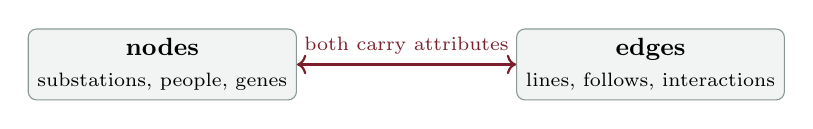
\begin{tikzpicture}[every node/.style={font=\small}]
    \node[draw=bgray, fill=fgray, rounded corners=3pt, minimum width=3.4cm, minimum height=0.9cm, align=center] (e) at (0,0) {\textbf{nodes}\\ \scriptsize substations, people, genes};
    \node[draw=bgray, fill=fgray, rounded corners=3pt, minimum width=3.4cm, minimum height=0.9cm, align=center] (r) at (6.2,0) {\textbf{edges}\\ \scriptsize lines, follows, interactions};
    \draw[<->, thick, burgundy] (e) -- node[above, font=\scriptsize\color{muted}]{both carry attributes} (r);
  \end{tikzpicture}
  \end{center}
  \vspace{0.2cm}
  \centering
  How is graph data managed at scale and in production?
\end{frame}

% ===== SLIDE 6: kinds of databases ============================================
\begin{frame}[fragile]{Three kinds of databases}
  \vspace{0.2cm}
  \begin{columns}[T]
    \column{0.32\textwidth}
      \begin{tbox}[Relational]{bslate}{fslate}
        Data in \textbf{tables} with fixed columns; rows reference each other by keys; queried with SQL. Relationships are computed with joins.\\[3pt]
        \kicker{PostgreSQL, MySQL, SQLite, DuckDB}
      \end{tbox}
      \vspace{0.1cm}
      \centering\scriptsize
      \begin{tabular}{@{}lll@{}}\toprule
        id & name & kv\\ \midrule
        S012 & Allegheny-12 & 345\\
        S036 & Laurel-01 & 345\\ \bottomrule
      \end{tabular}
    \column{0.32\textwidth}
      \begin{tbox}[Document (NoSQL)]{bgold}{fgold}
        Each record is a \textbf{JSON-like document} with its own shape; no fixed schema; fast to read and write whole records. Relationships are nested or referenced by id.\\[3pt]
        \kicker{MongoDB, CouchDB, DynamoDB}
      \end{tbox}
      \vspace{0.1cm}
      \begin{code}[json]
{ "id": "S012", "kv": 345,
  "lines": ["S036", "S016"] }
      \end{code}
    \column{0.32\textwidth}
      \begin{tbox}[Graph]{bgreen}{fgreen}
        \textbf{Nodes and relationships} are both stored; a relationship is a record pointing at its two ends. Queried by pattern.\\[3pt]
        \kicker{neo4j, Amazon Neptune, TigerGraph, Memgraph}
      \end{tbox}
      \vspace{0.1cm}
      \centering
      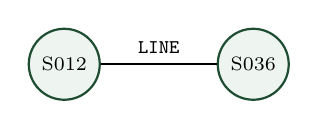
\begin{tikzpicture}[every node/.style={font=\scriptsize}, nd/.style={circle, draw=forest, fill=fgreen, thick, minimum size=0.75cm, align=center}]
        \node[nd] (a) at (0,0) {S012};
        \node[nd] (b) at (2.4,0) {S036};
        \draw[thick] (a) -- node[above]{\texttt{LINE}} (b);
      \end{tikzpicture}
  \end{columns}
\end{frame}

% ===== SLIDE 7: graph databases ===============================================
\begin{frame}[fragile]{Graph databases}
  \vspace{0.2cm}
  \begin{columns}[T]
    \column{0.55\textwidth}
      \small
      \begin{tabular}{@{}p{2.6cm}p{4.6cm}@{}}\toprule
        \textbf{neo4j} & The most widely used graph database. Property graph model, Cypher query language, open-source core, built-in algorithms library (GDS), desktop app, Docker image, cloud service (Aura).\\[4pt]
        Amazon Neptune & AWS-hosted; supports property graphs (openCypher, Gremlin) and RDF (SPARQL).\\[4pt]
        TigerGraph & Commercial, aimed at very large graphs and analytics; its own query language (GSQL).\\[4pt]
        Memgraph, ArangoDB, K\`uzu & Smaller or newer: in-memory, multi-model, or embedded.\\ \bottomrule
      \end{tabular}
    \column{0.43\textwidth}
      \begin{tbox}[Two data models]{bgray}{fgray}
        \textbf{Property graph}: nodes and relationships with labels and key--value properties (neo4j, Neptune, TigerGraph).\\[3pt]
        \textbf{RDF (Resource Description Framework) / triple store}: everything is a (subject, predicate, object) triple, queried with SPARQL (GraphDB, Virtuoso). Common in the semantic-web world.
      \end{tbox}
      \vspace{0.2cm}
      \small
      We'll use neo4j: it has the largest community and the most documentation.
  \end{columns}
\end{frame}

% ===== SLIDE 8: example data ==================================================
\begin{frame}[fragile]{Example data: a mock regional power grid}
  \vspace{0.1cm}
  \begin{columns}[T]
    \column{0.58\textwidth}
      \includegraphics[width=\textwidth]{../demo/figures/grid_map.pdf}
    \column{0.41\textwidth}
      \small
      \textbf{Nodes}
      \begin{itemize}
        \item \textbf{Generator} (25): type (gas, wind, solar, hydro, nuclear), capacity in MW, cost, on/off
        \item \textbf{Substation} (140): voltage level (345 / 138 / 69 kV), region, on/off, location
        \item \textbf{Load} (60): residential, industrial, or hospital; demand in MW
      \end{itemize}
      \textbf{Edges}
      \begin{itemize}
        \item \textbf{LINE} (322): substation to substation; capacity, length, annual fault probability
        \item \textbf{FEEDS} (25): generator to substation
        \item \textbf{SUPPLIES} (60): substation to load
      \end{itemize}
  \end{columns}
  \vspace{0.1cm}
  \kicker{Synthetic power grid built to mimic the Mid-Atlantic power grid, with five regions.}
\end{frame}

% ===== SLIDE 9: relational vs graph ===========================================
\begin{frame}[fragile]{The grid in a relational database and in neo4j}
  \vspace{0.1cm}
  \begin{columns}[T]
    \column{0.5\textwidth}
      \centering {\small\bfseries Relational: two tables, joined by keys}\\[4pt]
      {\scriptsize
      \begin{tabular}{@{}lll@{}}\toprule
        \multicolumn{3}{@{}l}{\texttt{substation}}\\ \midrule
        \texttt{id} & \texttt{name} & \texttt{kv}\\
        S012 & Allegheny-12 & 345\\
        S036 & Laurel-01 & 345\\
        S044 & Laurel-09 & 345\\ \bottomrule
      \end{tabular}\qquad
      \begin{tabular}{@{}lll@{}}\toprule
        \multicolumn{3}{@{}l}{\texttt{line}}\\ \midrule
        \texttt{from} & \texttt{to} & \texttt{fault\_prob}\\
        S012 & S036 & 0.07\\
        S036 & S044 & 0.03\\ \bottomrule
      \end{tabular}}\\[8pt]
      \begin{code}[SQL]
-- substations two lines away from S012
SELECT b.to
FROM line a JOIN line b ON a.to = b.from
WHERE a.from = 'S012';
      \end{code}
      \kicker{Each extra hop is another join over the whole \texttt{line} table.}
    \column{0.5\textwidth}
      \centering {\small\bfseries Graph: substations are nodes, lines are relationships}\\[8pt]
      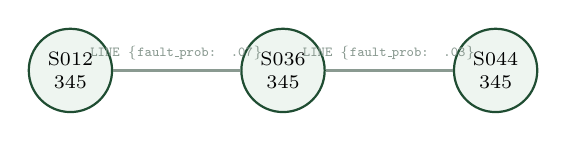
\begin{tikzpicture}[every node/.style={font=\scriptsize},
          sub/.style={circle, draw=forest, fill=fgreen, thick, minimum size=0.9cm, align=center}]
        \node[sub] (a) at (0,0) {S012\\345};
        \node[sub] (b) at (2.7,0) {S036\\345};
        \node[sub] (c) at (5.4,0) {S044\\345};
        \draw[thick, bgray] (a) -- node[above, font=\tiny]{\texttt{LINE \{fault\_prob: .07\}}} (b);
        \draw[thick, bgray] (b) -- node[above, font=\tiny]{\texttt{LINE \{fault\_prob: .03\}}} (c);
      \end{tikzpicture}\\[10pt]
      \begin{code}
// substations two lines away from S012
MATCH (a:Substation {id: 'S012'})
      -[:LINE]-()-[:LINE]-(b)
RETURN b
      \end{code}
      \kicker{The query is the picture: nodes in parentheses, relationships in brackets. Each hop follows stored pointers from the current node.}
  \end{columns}
\end{frame}

% ===== SLIDE 10: a first cypher query =========================================
\begin{frame}[fragile]{A first Cypher query}
  \vspace{0.2cm}
  \begin{columns}[T]
    \column{0.48\textwidth}
      \centering {\small\bfseries Look up one row}\\[4pt]
      \begin{code}[SQL]
SELECT *
FROM substation
WHERE name = 'Allegheny-01';
      \end{code}
      \begin{code}
MATCH (s:Substation {name: 'Allegheny-01'})
RETURN s
      \end{code}
      \small
      \begin{itemize}
        \item \texttt{MATCH} finds things, \texttt{RETURN} gives them back
        \item \texttt{(s:Substation \{\ldots\})} is one node: variable \texttt{s}, label \texttt{Substation}, a property filter
      \end{itemize}
    \column{0.48\textwidth}
      \centering {\small\bfseries Then one step further}\\[4pt]
      \begin{code}[SQL]
SELECT t.*
FROM substation s
JOIN line l       ON l.from = s.id
JOIN substation t ON t.id = l.to
WHERE s.name = 'Allegheny-01';
      \end{code}
      \begin{code}
MATCH (s:Substation {name: 'Allegheny-01'})-[:LINE]-(t)
RETURN t
      \end{code}
      \small
      \begin{itemize}
        \item \texttt{-[:LINE]-} is a relationship of type \texttt{LINE}, either direction (the SQL needs a union for that)
        \item the pattern reads the way the graph is drawn
      \end{itemize}
  \end{columns}
\end{frame}

% ===== SLIDE 11: property graph model =========================================
\begin{frame}[fragile]{The property graph model, with the grid}
  \vspace{0.3cm}
  \begin{center}
  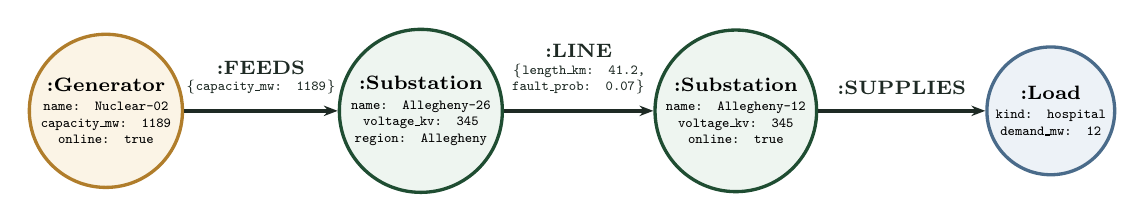
\begin{tikzpicture}[every node/.style={font=\tiny}, >={Stealth[length=5pt]},
      circ/.style={circle, very thick, minimum size=1.55cm, align=center, inner sep=1pt}]
    \node[circ, draw=bgold, fill=fgold] (g) at (0,0) {\textbf{\scriptsize :Generator}\\[1pt] \ttfamily name: Nuclear-02\\ \ttfamily capacity\_mw: 1189\\ \ttfamily online: true};
    \node[circ, draw=forest, fill=fgreen] (s) at (4.0,0) {\textbf{\scriptsize :Substation}\\[1pt] \ttfamily name: Allegheny-26\\ \ttfamily voltage\_kv: 345\\ \ttfamily region: Allegheny};
    \node[circ, draw=forest, fill=fgreen] (t) at (8.0,0) {\textbf{\scriptsize :Substation}\\[1pt] \ttfamily name: Allegheny-12\\ \ttfamily voltage\_kv: 345\\ \ttfamily online: true};
    \node[circ, draw=bslate, fill=fslate] (l) at (12.0,0) {\textbf{\scriptsize :Load}\\[1pt] \ttfamily kind: hospital\\ \ttfamily demand\_mw: 12};
    \draw[->, very thick, ink] (g) -- node[above=2pt, align=center]{\textbf{\scriptsize :FEEDS}\\ \ttfamily \{capacity\_mw: 1189\}} (s);
    \draw[->, very thick, ink] (s) -- node[above=2pt, align=center]{\textbf{\scriptsize :LINE}\\ \ttfamily \{length\_km: 41.2,\\ \ttfamily fault\_prob: 0.07\}} (t);
    \draw[->, very thick, ink] (t) -- node[above=2pt, align=center]{\textbf{\scriptsize :SUPPLIES}} (l);
  \end{tikzpicture}
  \end{center}
  \vspace{0.3cm}
  \begin{columns}[T]
    \column{0.32\textwidth}
      \begin{tbox}[Nodes]{bgreen}{fgreen}
        One or more \textbf{labels} (\texttt{:Substation}) and \textbf{properties}: numbers, strings, booleans, lists, dates, points.
      \end{tbox}
    \column{0.32\textwidth}
      \begin{tbox}[Relationships]{bgold}{fgold}
        Exactly one \textbf{type} (\texttt{:LINE}), a \textbf{direction}, and their own \textbf{properties}. Always join two existing nodes.
      \end{tbox}
    \column{0.32\textwidth}
      \begin{tbox}[Schema]{bslate}{fslate}
        Optional. No table definitions up front; constraints and indexes are added where needed. Mixed node types are normal.
      \end{tbox}
  \end{columns}
\end{frame}

% ===== SLIDE 12: the grid as a cypher pattern =================================
\begin{frame}[fragile]{The grid as a Cypher pattern}
  \vspace{0.1cm}
  \begin{columns}[T]
    \column{0.56\textwidth}
      \includegraphics[width=\textwidth]{../demo/figures/grid_map.pdf}
    \column{0.43\textwidth}
      \vspace{0.2cm}
      \begin{code}
(:Generator {type, capacity_mw,
             marginal_cost, online})
    -[:FEEDS {capacity_mw}]->
(:Substation {voltage_kv, region,
              online, lat, lon})
    -[:LINE {capacity_mw, length_km,
             fault_prob}]-
(:Substation)
    -[:SUPPLIES]->
(:Load {kind, demand_mw})
      \end{code}
      \small
      The whole data model fits in one pattern. A query is a piece of this pattern with some values filled in, for example "a nuclear generator, its substation, and the hospitals within three lines".
  \end{columns}
  \vspace{0.1cm}
  \kicker{Direction is stored (\texttt{FEEDS} goes generator $\to$ substation) and can be ignored when querying (\texttt{-[:LINE]-}).}
\end{frame}

% ===== SLIDE 13: when to use ==================================================
\begin{frame}[fragile]{When to use a graph database}
  \vspace{0.2cm}
  \begin{columns}[T]
    \column{0.48\textwidth}
      \begin{tbox}[Good fit]{bgreen}{fgreen}
        \begin{itemize}
          \item questions about \textbf{paths and neighborhoods}: within $k$ hops, is there a route, what connects A to B
          \item \textbf{many entity types} with relationships among them, and a schema that keeps changing
          \item the graph is \textbf{larger than memory} or used by several people and services at once
          \item queries, indexes, transactions, and graph algorithms on one copy of the data
        \end{itemize}
      \end{tbox}
    \column{0.48\textwidth}
      \begin{tbox}[Poor fit]{bburg}{fburg}
        \begin{itemize}
          \item \textbf{column aggregates} over millions of rows: relational and columnar databases are faster
          \item a graph that \textbf{fits in memory}, analyzed once: \texttt{networkx}, \texttt{igraph}, or \texttt{graph-tool} are simpler and faster
          \item tabular analyses with one or two joins
          \item work that needs the \textbf{adjacency matrix} itself
        \end{itemize}
      \end{tbox}
  \end{columns}
  \vspace{0.4cm}
  \centering
  A graph database is a \textbf{storage and query} decision.
\end{frame}

% ===== SLIDE 14: how neo4j stores a graph =====================================
\begin{frame}[fragile]{How neo4j stores a graph}
  \vspace{0.1cm}
  \begin{columns}[T]
    \column{0.55\textwidth}
      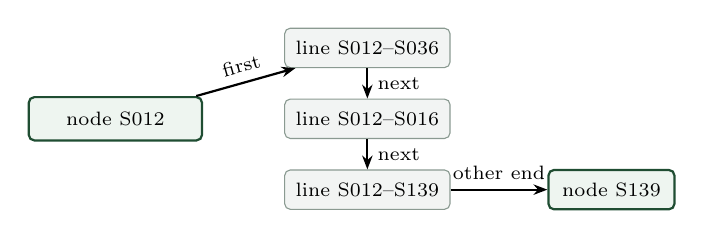
\begin{tikzpicture}[every node/.style={font=\scriptsize}, >={Stealth[length=5pt]}]
        \node[draw=forest, fill=fgreen, thick, rounded corners=2pt, minimum width=2.2cm, minimum height=0.55cm] (n) at (0,0) {node S012};
        \node[draw=bgray, fill=fgray, rounded corners=2pt, minimum width=2.1cm, minimum height=0.5cm] (r1) at (3.2,0.9) {line S012--S036};
        \node[draw=bgray, fill=fgray, rounded corners=2pt, minimum width=2.1cm, minimum height=0.5cm] (r2) at (3.2,0) {line S012--S016};
        \node[draw=bgray, fill=fgray, rounded corners=2pt, minimum width=2.1cm, minimum height=0.5cm] (r3) at (3.2,-0.9) {line S012--S139};
        \node[draw=forest, fill=fgreen, thick, rounded corners=2pt, minimum width=1.6cm, minimum height=0.5cm] (m) at (6.3,-0.9) {node S139};
        \draw[->, thick] (n) -- node[above, sloped]{first} (r1);
        \draw[->, thick] (r1) -- node[right]{next} (r2);
        \draw[->, thick] (r2) -- node[right]{next} (r3);
        \draw[->, thick] (r3) -- node[above]{other end} (m);
      \end{tikzpicture}\\[6pt]
      \small
      Every node record holds a pointer to its first relationship; relationships are chained in a list and each one points at both of its end nodes. Moving to a neighbor means following a pointer.
    \column{0.43\textwidth}
      \small
      \textbf{What this buys}
      \begin{itemize}
        \item a hop costs the same whether the graph has a thousand nodes or a billion
        \item a $k$-hop query touches only the part of the graph it walks through
      \end{itemize}
      \vspace{0.2cm}
      \textbf{What it does not}
      \begin{itemize}
        \item finding the \emph{starting} node ("the substation named X") still needs an index, which you create with a constraint
        \item writes are a little slower, because the lists have to be maintained
      \end{itemize}
  \end{columns}
\end{frame}

% ===== PART 2 =================================================================
\partslide{02}{Setup and Cypher}

% ===== SLIDE 16: setup ========================================================
\begin{frame}[fragile]{Setting up your own database}
  \vspace{0.1cm}
  \begin{columns}[T]
    \column{0.5\textwidth}
      \begin{tbox}[Docker (used today)]{bgreen}{fgreen}
        \begin{code}[bash]
cd demo && docker compose up -d
# then open http://localhost:7474
        \end{code}
        Port \texttt{7474} is the Browser, \texttt{7687} the driver port; \texttt{./data} is mounted at \texttt{/import}.
      \end{tbox}
      \begin{code}[yaml]
services:
  neo4j:
    image: neo4j:5
    ports: ["7474:7474", "7687:7687"]
    environment:
      NEO4J_AUTH: neo4j/statbytes2026
      NEO4J_PLUGINS: '["graph-data-science"]'
    volumes: ["./data:/import"]
      \end{code}
    \column{0.5\textwidth}
      \begin{tbox}[Neo4j Desktop (no Docker)]{bslate}{fslate}
        1. Download from \texttt{neo4j.com/download}\\
        2. Add $\to$ Local DBMS, choose a password\\
        3. Plugins tab $\to$ install Graph Data Science\\
        4. Copy the CSVs into the DBMS's \texttt{import} folder\\
        5. Start, open Browser
      \end{tbox}
      \begin{tbox}[Aura (hosted)]{bgold}{fgold}
        Free tier, nothing to install. No GDS on the free tier (AuraDS is the paid option). Fine for the Cypher part of this talk.
      \end{tbox}
  \end{columns}
\end{frame}

% ===== SLIDE 17: loading data =================================================
\begin{frame}[fragile]{Loading data}
  \vspace{0.1cm}
  \begin{columns}[T]
    \column{0.52\textwidth}
      \begin{code}
// a uniqueness constraint also creates an index
CREATE CONSTRAINT sub_id IF NOT EXISTS
  FOR (s:Substation) REQUIRE s.id IS UNIQUE;

// nodes: one CSV row -> one node
LOAD CSV WITH HEADERS
  FROM 'file:///substations.csv' AS row
CREATE (:Substation {
  id: row.id, name: row.name,
  voltage_kv: toInteger(row.voltage_kv),
  region: row.region,
  online: toBoolean(row.online)
});
      \end{code}
    \column{0.46\textwidth}
      \begin{code}
// relationships: find both ends, connect them
LOAD CSV WITH HEADERS
  FROM 'file:///lines.csv' AS row
MATCH (a:Substation {id: row.from_id}),
      (b:Substation {id: row.to_id})
CREATE (a)-[:LINE {
  capacity_mw: toInteger(row.capacity_mw),
  length_km:   toFloat(row.length_km),
  fault_prob:  toFloat(row.fault_prob)
}]->(b);
      \end{code}
      \small
      \begin{itemize}
        \item CSV values arrive as strings; cast them
        \item the \texttt{MATCH} on \texttt{id} uses the index from the constraint
        \item for very large files: \texttt{neo4j-admin database import}, or batched writes from a driver
      \end{itemize}
  \end{columns}
  \vspace{0.1cm}
  \kicker{The full script is \texttt{cypher/01\_load.cypher}: three constraints, six \texttt{LOAD CSV} blocks, one count at the end.}
\end{frame}

% ===== SLIDE 18: intro to cypher ==============================================
\begin{frame}[fragile]{Cypher queries}
  \vspace{0.1cm}
  \begin{code}
MATCH (g:Generator {type: 'nuclear'})-[:FEEDS]->(s:Substation)-[:LINE*1..3]-(t:Substation)
WHERE t.online AND t.voltage_kv >= 138
RETURN g.name, t.region, count(DISTINCT t) AS reachable
ORDER BY reachable DESC
  \end{code}
  \vspace{-0.1cm}
  {\small
  \begin{tabular}{@{}lp{7.2cm}@{}}
    \textcolor{bgreen}{\rule{6pt}{6pt}}\ \texttt{(g:Generator \{type: 'nuclear'\})} & a node: variable, label, property filter\\
    \textcolor{bgold}{\rule{6pt}{6pt}}\ \texttt{-[:FEEDS]->} & a relationship with a type and a direction\\
    \textcolor{bburg}{\rule{6pt}{6pt}}\ \texttt{-[:LINE*1..3]-} & one to three hops, either direction\\
    \textcolor{bslate}{\rule{6pt}{6pt}}\ \texttt{WHERE} \ldots \texttt{RETURN} \ldots \texttt{ORDER BY} & filter, project, aggregate; the non-aggregated columns are the groups\\
  \end{tabular}}
  \vspace{0.2cm}
  \begin{columns}[T]
    \column{0.32\textwidth}
      \begin{tbox}[Reading]{bgreen}{fgreen}
        \texttt{MATCH} a pattern, \texttt{WHERE} to filter, \texttt{RETURN} to project. \texttt{WITH} passes rows to another \texttt{MATCH}.
      \end{tbox}
    \column{0.32\textwidth}
      \begin{tbox}[Writing]{bgold}{fgold}
        \texttt{CREATE}, \texttt{MERGE} (create if missing), \texttt{SET}, \texttt{DELETE}. The same pattern syntax.
      \end{tbox}
    \column{0.32\textwidth}
      \begin{tbox}[Paths]{bslate}{fslate}
        \texttt{p = (a)-[*]-(b)} binds a path; \texttt{nodes(p)}, \texttt{length(p)}, \texttt{shortestPath()}. Bound variable-length patterns.
      \end{tbox}
  \end{columns}
\end{frame}

% ===== SLIDE 19: live cypher ==================================================
\begin{frame}[fragile]{Live: eight queries}
  \vspace{0.15cm}
  \footnotesize
  \begin{tabular}{@{}cp{3.8cm}p{7.5cm}@{}}\toprule
    & \textbf{Query} & \textbf{What it shows}\\ \midrule
    Q1 & counts by label and type & the shape of the data: \texttt{labels(n)}, \texttt{type(r)}\\
    Q2 & look up Allegheny-01 & a lookup; the same thing as \texttt{SELECT \ldots WHERE}\\
    Q3 & its neighbors, as a path & \texttt{RETURN p} and the Browser draws the result\\
    Q4 & nuclear plant, substation, one line out & three node types in one pattern\\
    Q5 & generation vs demand by region & \texttt{WITH} chains two matches; aggregates\\
    Q6 & hospitals within 3 lines of a nuclear plant & \texttt{[:LINE*1..3]}, \texttt{DISTINCT}\\
    Q7 & \texttt{shortestPath()} Allegheny-01 to Pocono-01 & path variables, \texttt{nodes(p)}\\
    Q8 & set an \texttt{inspected} date & a write, with the same syntax\\ \bottomrule
  \end{tabular}
  \vspace{0.4cm}
  \begin{tbox}[Browser tips]{bgray}{fgray}
    \texttt{Ctrl+Enter} runs. The result panel switches between graph, table, and text. \texttt{:schema} lists constraints. \texttt{EXPLAIN} or \texttt{PROFILE} in front of a query shows the plan.
  \end{tbox}
\end{frame}

% ===== SLIDE 20: python =======================================================
\begin{frame}[fragile]{Using Python with neo4j}
  \vspace{0.1cm}
  \begin{columns}[T]
    \column{0.52\textwidth}
      \begin{codesmall}[Python]
# pip install neo4j graphdatascience
from graphdatascience import GraphDataScience

URI, AUTH = "bolt://localhost:7687", ("neo4j", "statbytes2026")
gds = GraphDataScience(URI, auth=AUTH)
q = gds.run_cypher   # returns a DataFrame

query = """MATCH (s:Substation)-[:SUPPLIES]->(l:Load)
           WHERE s.region = $region
           RETURN l.kind, sum(l.demand_mw) AS mw"""
df = q(query, {"region": "Pocono"})
      \end{codesmall}
      \begin{codesmall}[Python]
# the plain driver, without the GDS client
from neo4j import GraphDatabase
drv = GraphDatabase.driver(URI, auth=AUTH)
df = drv.execute_query(query, region="Pocono",
        result_transformer_=lambda r: r.to_df())
      \end{codesmall}
    \column{0.46\textwidth}
      \small
      \begin{itemize}
        \item the connection is over \textbf{Bolt} (the protocol Python and neo4j use to communicate); the same code works for a local container, a server, or Aura
        \item \textbf{parameters} (\texttt{\$region}) keep the query text fixed
        \item every result is a \textbf{DataFrame}
        \item send the question to the database and get a summary back; for local algorithms, pull an edge list once
      \end{itemize}
  \end{columns}
\end{frame}

% ===== SLIDE 21: where the database lives =====================================
\begin{frame}[fragile]{In practice: where the database lives}
  \vspace{0.2cm}
  \begin{center}
  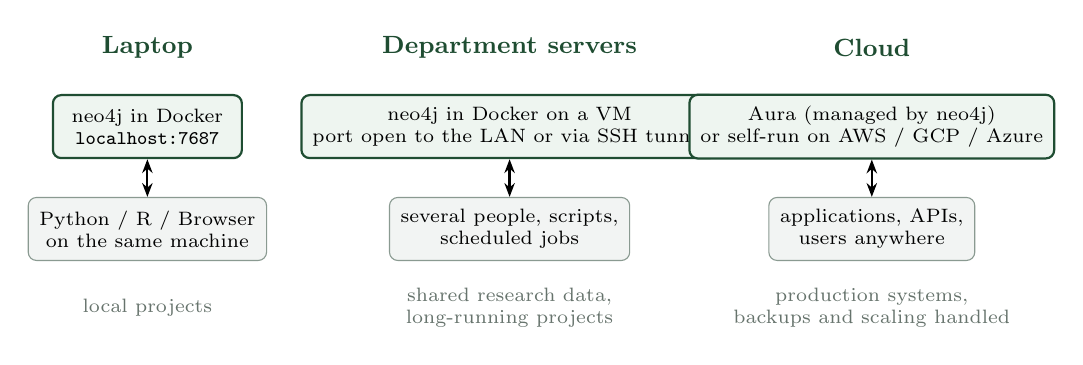
\begin{tikzpicture}[every node/.style={font=\scriptsize, align=center}, >={Stealth[length=5pt]},
      box/.style={draw=bgray, fill=fgray, rounded corners=3pt, minimum height=0.8cm, minimum width=2.4cm, inner sep=4pt},
      db/.style={draw=forest, fill=fgreen, thick, rounded corners=3pt, minimum height=0.8cm, minimum width=2.4cm, inner sep=4pt},
      hdr/.style={font=\small\bfseries\color{forest}}]
    % column 1: laptop
    \node[hdr] at (0,2.3) {Laptop};
    \node[db] (l1) at (0,1.3) {neo4j in Docker\\ \texttt{localhost:7687}};
    \node[box] (l2) at (0,0) {Python / R / Browser\\ on the same machine};
    \draw[<->, thick] (l1) -- (l2);
    \node[text=muted] at (0,-1.0) {local projects};
    % column 2: server
    \node[hdr] at (4.6,2.3) {Department servers};
    \node[db] (s1) at (4.6,1.3) {neo4j in Docker on a VM\\ port open to the LAN or via SSH tunnel};
    \node[box] (s2) at (4.6,0) {several people, scripts,\\ scheduled jobs};
    \draw[<->, thick] (s1) -- (s2);
    \node[text=muted] at (4.6,-1.0) {shared research data,\\ long-running projects};
    % column 3: cloud
    \node[hdr] at (9.2,2.3) {Cloud};
    \node[db] (c1) at (9.2,1.3) {Aura (managed by neo4j)\\ or self-run on AWS / GCP / Azure};
    \node[box] (c2) at (9.2,0) {applications, APIs,\\ users anywhere};
    \draw[<->, thick] (c1) -- (c2);
    \node[text=muted] at (9.2,-1.0) {production systems,\\ backups and scaling handled};
  \end{tikzpicture}
  \end{center}
  \vspace{0.2cm}
  \small
  \begin{itemize}
    \item The code is the same in all three: a Bolt URL, a user, a password.
  \end{itemize}
\end{frame}

% ===== SLIDE 22: backend for an app ===========================================
\begin{frame}[fragile]{In practice: a graph database behind a web application}
  \vspace{0.2cm}
  \begin{center}
  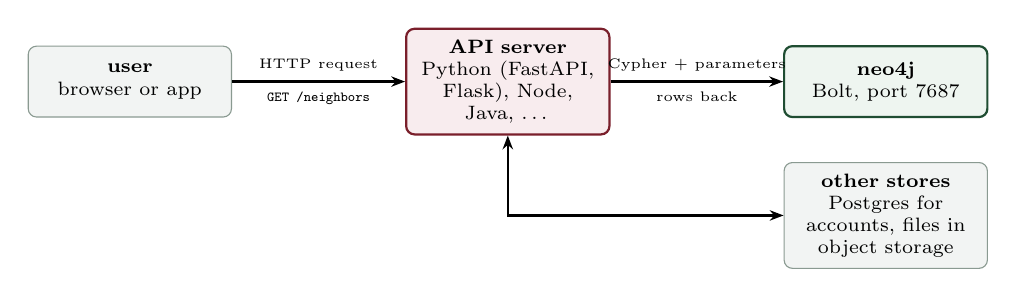
\begin{tikzpicture}[every node/.style={font=\scriptsize, align=center}, >={Stealth[length=5pt]},
      box/.style={draw=bgray, fill=fgray, rounded corners=3pt, minimum height=0.9cm, text width=2.3cm, inner sep=4pt},
      db/.style={draw=forest, fill=fgreen, thick, rounded corners=3pt, minimum height=0.9cm, text width=2.3cm, inner sep=4pt},
      hi/.style={draw=burgundy, fill=fburg, thick, rounded corners=3pt, minimum height=0.9cm, text width=2.3cm, inner sep=4pt}]
    \node[box] (u) at (0,0) {\textbf{user}\\ browser or app};
    \node[hi] (api) at (4.8,0) {\textbf{API server}\\ Python (FastAPI, Flask), Node, Java, \ldots};
    \node[db] (db) at (9.6,0) {\textbf{neo4j}\\ Bolt, port 7687};
    \node[box] (other) at (9.6,-1.7) {\textbf{other stores}\\ Postgres for accounts, files in object storage};
    \draw[->, thick] (u) -- node[above, font=\tiny]{HTTP request} node[below, font=\tiny]{\texttt{GET /neighbors}} (api);
    \draw[->, thick] (api) -- node[above, font=\tiny]{Cypher + parameters} node[below, font=\tiny]{rows back} (db);
    \draw[<->, thick] (api) |- (other);
  \end{tikzpicture}
  \end{center}
  \vspace{0.15cm}
  \begin{columns}[T]
    \column{0.48\textwidth}
      \small
      \textbf{The usual pattern}
      \begin{itemize}
        \item the API server holds a pool of driver connections and a read-only database user; users never reach the database directly
        \item each endpoint is one Cypher query with parameters; results go back as JSON
        \item GDS jobs run on a schedule and write results back; endpoints only read
      \end{itemize}
    \column{0.48\textwidth}
      \small
      \textbf{Typical uses}
      \begin{itemize}
        \item recommendations: people who bought this also bought
        \item fraud: rings of accounts sharing devices and addresses
        \item network operations and digital twins: outages, dependencies, what-if
      \end{itemize}
  \end{columns}
\end{frame}

% ===== PART 3 =================================================================
\partslide{03}{Graph Data Science}

% ===== SLIDE 24: GDS overview =================================================
\begin{frame}[fragile]{The Graph Data Science library}
  \vspace{0.1cm}
  \begin{center}
  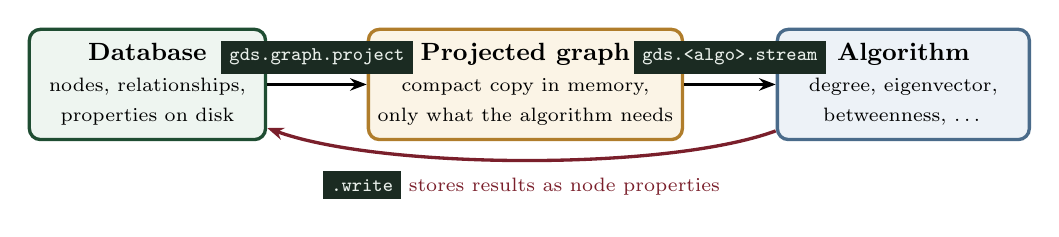
\begin{tikzpicture}[every node/.style={font=\small}, >={Stealth[length=6pt]}]
    \node[draw=forest, fill=fgreen, very thick, rounded corners=4pt, minimum width=3cm, minimum height=1.4cm, align=center] (db) at (0,0) {\textbf{Database}\\ \scriptsize nodes, relationships,\\ \scriptsize properties on disk};
    \node[draw=bgold, fill=fgold, very thick, rounded corners=4pt, minimum width=3.4cm, minimum height=1.4cm, align=center] (proj) at (4.8,0) {\textbf{Projected graph}\\ \scriptsize compact copy in memory,\\ \scriptsize only what the algorithm needs};
    \node[draw=bslate, fill=fslate, very thick, rounded corners=4pt, minimum width=3.2cm, minimum height=1.4cm, align=center] (alg) at (9.6,0) {\textbf{Algorithm}\\ \scriptsize degree, eigenvector,\\ \scriptsize betweenness, \ldots};
    \draw[->, very thick] (db) -- node[above]{\chip{gds.graph.project}} (proj);
    \draw[->, very thick] (proj) -- node[above]{\chip{gds.<algo>.stream}} (alg);
    \draw[->, very thick, burgundy] (alg) to[out=-160, in=-20, looseness=0.6] node[below, font=\scriptsize]{\chip{.write} stores results as node properties} (db);
  \end{tikzpicture}
  \end{center}
  \vspace{0.1cm}
  \begin{columns}[T]
    \column{0.5\textwidth}
      \begin{code}
CALL gds.graph.project('grid', 'Substation',
  { LINE: { orientation: 'UNDIRECTED' } });

CALL gds.degree.stream('grid')
YIELD nodeId, score
RETURN gds.util.asNode(nodeId).name, score
ORDER BY score DESC LIMIT 10;
      \end{code}
    \column{0.48\textwidth}
      \small
      \begin{itemize}
        \item a plugin that runs inside the database; called from Cypher with \texttt{CALL gds.\ldots}
        \item most algorithms have four modes: \texttt{stream} (rows back), \texttt{stats}, \texttt{mutate} (update the projection), \texttt{write} (update the database)
      \end{itemize}
  \end{columns}
\end{frame}

% ===== SLIDE 25: algorithm families ===========================================
\begin{frame}[fragile]{What is in the library}
  \vspace{0.2cm}
  \begin{columns}[T]
    \column{0.24\textwidth}
      \begin{tbox}[Centrality]{bgreen}{fgreen}
        degree, eigenvector, PageRank, betweenness, closeness\\[3pt]
        \emph{which nodes are important?}
      \end{tbox}
    \column{0.24\textwidth}
      \begin{tbox}[Community and components]{bgold}{fgold}
        connected components, Louvain, Leiden, label propagation, triangle counts\\[3pt]
        \emph{what are the groups?}
      \end{tbox}
    \column{0.24\textwidth}
      \begin{tbox}[Paths]{bslate}{fslate}
        shortest paths (Dijkstra, A*), $k$ shortest paths, spanning trees, random walks\\[3pt]
        \emph{how do I get from A to B?}
      \end{tbox}
    \column{0.24\textwidth}
      \begin{tbox}[Similarity, embeddings, ML]{bburg}{fburg}
        node similarity, $k$-nearest neighbors, FastRP and node2vec embeddings, link prediction pipelines\\[3pt]
        \emph{which nodes are alike?}
      \end{tbox}
  \end{columns}
  \vspace{0.6cm}
  \centering
  GDS documentation provides a description and the requirements of each algorithm.
\end{frame}

% ===== SLIDE 26: projections ==================================================
\begin{frame}[fragile]{Graph projections: what and why}
  \vspace{0.1cm}
  \begin{columns}[T]
    \column{0.5\textwidth}
      \begin{code}
// native projection: labels and relationship types
CALL gds.graph.project(
  'grid',                      // a name
  'Substation',                // which nodes
  { LINE: { orientation: 'UNDIRECTED' } }
)
YIELD nodeCount, relationshipCount;
// -> 140 nodes, 644 relationships

// Cypher projection: any pattern you can write
MATCH (s:Substation)-[:LINE]-(t:Substation)
WHERE s.online AND t.online
RETURN gds.graph.project('grid_online', s, t);
      \end{code}
    \column{0.48\textwidth}
      \small
      \textbf{What it is.} A copy of part of the graph in a compact in-memory format, with a name. Algorithms run on the projection, never on the stored data.\\[4pt]
      \textbf{Why.}
      \begin{itemize}
        \item algorithms need the whole graph in a form built for fast iteration; the storage format is built for lookups and updates
        \item you choose the subgraph: only substations and lines, only online nodes, only one region
        \item you choose the direction: \texttt{UNDIRECTED} for a grid, \texttt{NATURAL} for a citation network
        \item one projection serves many algorithms, then is dropped
      \end{itemize}
      \kicker{Undirected lines are stored both ways, so 322 lines become 644 relationships.}
  \end{columns}
\end{frame}

% ===== SLIDE 27: degree =======================================================
\begin{frame}[fragile]{Degree centrality}
  \vspace{0.1cm}
  \begin{columns}[T]
    \column{0.46\textwidth}
      \small
      The number of edges at a node. With the adjacency matrix $A$,
      \[ d_i = \sum_{j} A_{ij}. \]
      Directed graphs have an in-degree (column sum) and an out-degree (row sum). With weights, the sum of the weights.\\[5pt]
      \textbf{What it says.} How many direct connections a node has; for the grid, how many lines meet at a substation.\\[5pt]
      \textbf{Limits.} Purely local. Eight lines to dead ends score the same as eight lines to other hubs.
    \column{0.52\textwidth}
      \begin{code}
CALL gds.degree.stream('grid')
YIELD nodeId, score
WITH gds.util.asNode(nodeId) AS s, score
RETURN s.name, s.region, toInteger(score) AS degree
ORDER BY score DESC LIMIT 10;
      \end{code}
      \begin{codesmall}[Python]
df = q("CALL gds.degree.stream('grid') YIELD nodeId, score "
       "RETURN gds.util.asNode(nodeId).name AS name, score")
      \end{codesmall}
      \kicker{Options: \texttt{orientation} and \texttt{relationshipWeightProperty} (weighted degree).}
  \end{columns}
\end{frame}

% ===== SLIDE 28: eigenvector ==================================================
\begin{frame}[fragile]{Eigenvector centrality}
  \vspace{0.1cm}
  \begin{columns}[T]
    \column{0.46\textwidth}
      \small
      A node scores high if its neighbors score high. Each score is proportional to the sum of its neighbors' scores:
      \[ x_i = \frac{1}{\lambda}\sum_j A_{ij}\, x_j \quad\Longleftrightarrow\quad A\,x = \lambda\, x . \]
      $x$ is the leading eigenvector of $A$; for a connected graph it is unique and positive.\\[5pt]
      \textbf{What it says.} Connections to well-connected nodes count for more than raw degree. PageRank is a damped variant for directed graphs.\\[5pt]
      \textbf{Limits.} Dominated by the densest cluster; with weakly joined regions, one region can take all the mass.
    \column{0.52\textwidth}
      \begin{code}
CALL gds.eigenvector.stream('grid', { maxIterations: 200 })
YIELD nodeId, score
WITH gds.util.asNode(nodeId) AS s, score
RETURN s.name, s.region, round(score, 3) AS eigenvector
ORDER BY score DESC LIMIT 10;
      \end{code}
      \begin{codesmall}[Python]
df = q("CALL gds.eigenvector.stream('grid') YIELD nodeId, score "
       "RETURN gds.util.asNode(nodeId).name AS name, score")
      \end{codesmall}
      \kicker{Options: \texttt{maxIterations}, \texttt{tolerance}, \texttt{scaler}. By default the returned vector has unit length (L2 norm 1).}
  \end{columns}
\end{frame}

% ===== SLIDE 29: betweenness ==================================================
\begin{frame}[fragile]{Betweenness centrality}
  \vspace{0.1cm}
  \begin{columns}[T]
    \column{0.46\textwidth}
      \small
      The share of shortest paths that pass through a node. With $\sigma_{st}$ the number of shortest paths from $s$ to $t$ and $\sigma_{st}(v)$ the number of those that go through $v$,
      \[ b_v = \sum_{s \neq v \neq t} \frac{\sigma_{st}(v)}{\sigma_{st}} . \]
      Computed with Brandes' algorithm: one breadth-first search per source node, $O(nm)$ in total.\\[5pt]
      \textbf{What it says.} Which nodes sit on the routes between other nodes; for the grid, which substations carry traffic between regions.\\[5pt]
      \textbf{Limits.} Assumes flow follows shortest paths. Cost grows fast with size; GDS has a sampled version (\texttt{samplingSize}).
    \column{0.52\textwidth}
      \begin{code}
CALL gds.betweenness.stream('grid')
YIELD nodeId, score
WITH gds.util.asNode(nodeId) AS s, score
RETURN s.name, s.region, round(score) AS betweenness
ORDER BY score DESC LIMIT 10;
      \end{code}
      \begin{codesmall}[Python]
df = q("CALL gds.betweenness.stream('grid') YIELD nodeId, score "
       "RETURN gds.util.asNode(nodeId).name AS name, score")
      \end{codesmall}
      \kicker{GDS returns raw path counts. Divide by $(n-1)(n-2)/2$ for the usual $[0,1]$ scale on an undirected graph.}
  \end{columns}
\end{frame}

% ===== SLIDE 30: in practice: degree ==========================================
\begin{frame}[fragile]{In practice: degree}
  \vspace{0.1cm}
  \begin{columns}[T]
    \column{0.58\textwidth}
      \includegraphics[width=\textwidth]{../demo/figures/degree.pdf}
    \column{0.41\textwidth}
      {\footnotesize
      \begin{tabular}{@{}llrr@{}}\toprule
        substation & region & kV & degree\\ \midrule
        Allegheny-12 & Allegheny & 345 & 8\\
        Allegheny-14 & Allegheny & 69 & 8\\
        Laurel-02 & Laurel & 69 & 8\\
        Susquehanna-27 & Susquehanna & 345 & 8\\
        Pocono-08 & Pocono & 345 & 7\\
        Pocono-11 & Pocono & 138 & 7\\ \bottomrule
      \end{tabular}}
      \vspace{0.3cm}
      \small
      \begin{itemize}
        \item projection: 140 nodes, 644 relationships
        \item the top of the list mixes 345 kV hubs with 69 kV substations that happen to have many short local lines
        \item degree alone does not separate "important for the grid" from "many small connections"
      \end{itemize}
  \end{columns}
\end{frame}

% ===== SLIDE 31: in practice: eigenvector =====================================
\begin{frame}[fragile]{In practice: eigenvector}
  \vspace{0.1cm}
  \begin{columns}[T]
    \column{0.58\textwidth}
      \includegraphics[width=\textwidth]{../demo/figures/eigenvector.pdf}
    \column{0.41\textwidth}
      {\footnotesize
      \begin{tabular}{@{}llrr@{}}\toprule
        substation & region & kV & score\\ \midrule
        Pocono-23 & Pocono & 69 & 0.353\\
        Pocono-16 & Pocono & 69 & 0.331\\
        Pocono-08 & Pocono & 345 & 0.329\\
        Pocono-15 & Pocono & 69 & 0.322\\
        Pocono-28 & Pocono & 69 & 0.283\\
        Pocono-05 & Pocono & 69 & 0.278\\ \bottomrule
      \end{tabular}}
      \vspace{0.3cm}
      \small
      \begin{itemize}
        \item the whole top ten is in Pocono, the most densely connected region
        \item this is the limit from the previous slide: the leading eigenvector concentrates on the densest cluster
        \item useful within one region; misleading as a grid-wide ranking
      \end{itemize}
  \end{columns}
\end{frame}

% ===== SLIDE 32: in practice: betweenness =====================================
\begin{frame}[fragile]{In practice: betweenness}
  \vspace{0.1cm}
  \begin{columns}[T]
    \column{0.58\textwidth}
      \includegraphics[width=\textwidth]{../demo/figures/betweenness.pdf}
    \column{0.41\textwidth}
      {\footnotesize
      \begin{tabular}{@{}llrr@{}}\toprule
        substation & region & kV & score\\ \midrule
        Susquehanna-27 & Susquehanna & 345 & 5171\\
        Erie-06 & Erie & 345 & 3871\\
        Allegheny-12 & Allegheny & 345 & 3600\\
        Erie-23 & Erie & 345 & 3431\\
        Pocono-06 & Pocono & 345 & 3038\\
        Susquehanna-03 & Susquehanna & 69 & 1939\\ \bottomrule
      \end{tabular}}
      \vspace{0.3cm}
      \small
      \begin{itemize}
        \item the top five are all 345 kV substations at the ends of the inter-ties between regions
        \item this is the ranking that matches "which substation would hurt most if it failed"
        \item Susquehanna-27 is on more than half of all shortest paths between pairs of substations (5171 of 9591)
      \end{itemize}
  \end{columns}
\end{frame}

% ===== SLIDE 33: what if a node broke =========================================
\begin{frame}[fragile]{What if a node broke? Connected components}
  \vspace{0.1cm}
  \begin{columns}[T]
    \column{0.52\textwidth}
      \includegraphics[width=\textwidth]{../demo/figures/islanding.pdf}\\[2pt]
      \centering
      {\scriptsize
      \begin{tabular}{@{}rlrrr@{}}\toprule
        subs & regions & gen & demand & hosp.\\ \midrule
        82 & Allegheny, Erie, Laurel & 5474 & 2807 & 4\\
        57 & Pocono, Susquehanna & 1488 & 1436 & 2\\ \bottomrule
      \end{tabular}}
    \column{0.47\textwidth}
      \begin{code}
MATCH (s:Substation {name: 'Susquehanna-27'})
SET s.online = false;
MATCH (s:Substation)-[:LINE]-(t:Substation)
WHERE s.online AND t.online
RETURN gds.graph.project('grid_online', s, t);
CALL gds.wcc.stream('grid_online')
YIELD nodeId, componentId ...
      \end{code}
      \small
      \textbf{Weakly connected components}: the groups of nodes that can reach each other by some path, ignoring direction. Each group is an electrical island.\\[4pt]
      \textbf{What we learn.} One substation splits the grid in two. The eastern island keeps 1488 MW of generation for 1436 MW of demand and two hospitals, which leaves little margin.
  \end{columns}
\end{frame}

% ===== PART 4 =================================================================
\partslide{04}{Knowledge graphs and RAG}

% ===== SLIDE 35: knowledge graphs =============================================
\begin{frame}[fragile]{Knowledge graphs}
  \vspace{0.15cm}
  \begin{columns}[T]
    \column{0.5\textwidth}
      \vspace{0.2cm}
      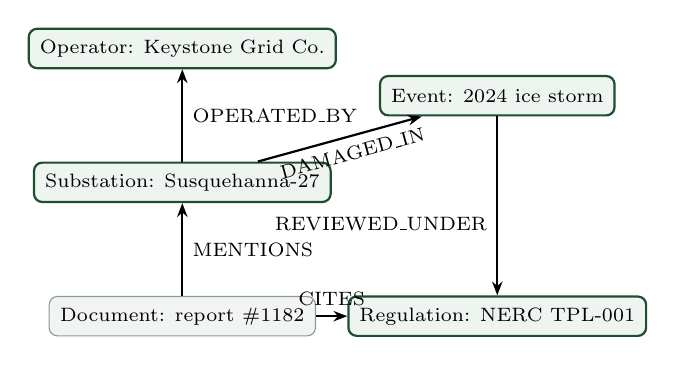
\begin{tikzpicture}[every node/.style={font=\scriptsize}, >={Stealth[length=5pt]},
          ent/.style={draw=forest, fill=fgreen, thick, rounded corners=3pt, minimum height=0.5cm, inner sep=4pt},
          doc/.style={draw=bgray, fill=fgray, rounded corners=3pt, minimum height=0.5cm, inner sep=4pt}]
        \node[ent] (a) at (0,0) {Substation: Susquehanna-27};
        \node[ent] (b) at (0,1.7) {Operator: Keystone Grid Co.};
        \node[ent] (c) at (4.0,1.1) {Event: 2024 ice storm};
        \node[doc] (d) at (0,-1.7) {Document: report \#1182};
        \node[ent] (e) at (4.0,-1.7) {Regulation: NERC TPL-001};
        \draw[->, thick] (a) -- node[right]{OPERATED\_BY} (b);
        \draw[->, thick] (a) -- node[below, sloped, pos=0.55]{DAMAGED\_IN} (c);
        \draw[->, thick] (d) -- node[right]{MENTIONS} (a);
        \draw[->, thick] (d) -- node[above]{CITES} (e);
        \draw[->, thick] (c) -- node[left, pos=0.6]{REVIEWED\_UNDER} (e);
      \end{tikzpicture}
    \column{0.48\textwidth}
      \small
      A \textbf{knowledge graph} is a property graph whose nodes are real-world entities and whose relationships are facts about them. Three things usually come with it:
      \begin{itemize}
        \item \textbf{schema (ontology)}: the allowed entity types and relationship types, sometimes with a hierarchy
        \item \textbf{provenance}: which document or source asserted each fact, and when
        \item \textbf{identity resolution}: "Susquehanna-27", "SUSQ27", and "the Milton substation" are one node
      \end{itemize}
      \vspace{0.1cm}
      Examples: Wikidata, Google's Knowledge Graph, Hetionet, digital twins of grids and factories.
  \end{columns}
  \vspace{0.15cm}
  \kicker{Language models read text well and recall exact facts unreliably. A knowledge graph keeps the facts; a language model can help build one from text.}
\end{frame}

% ===== SLIDE 36: RAG ==========================================================
\begin{frame}[fragile]{Retrieval-augmented generation (RAG)}
  \vspace{0.2cm}
  \begin{center}
  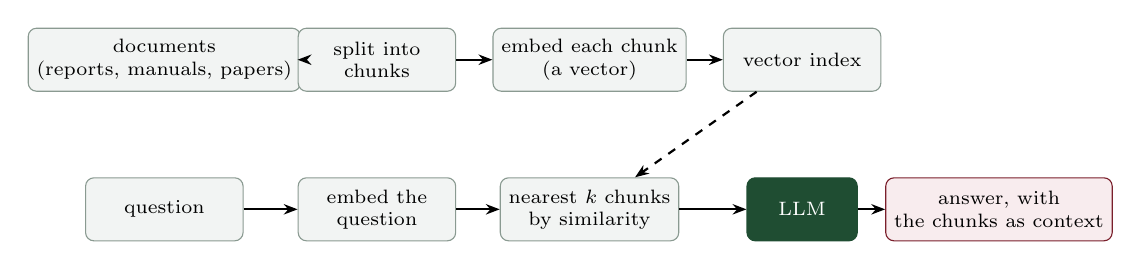
\begin{tikzpicture}[every node/.style={font=\scriptsize, align=center}, >={Stealth[length=5pt]},
      st/.style={draw=bgray, fill=fgray, rounded corners=3pt, minimum height=0.8cm, minimum width=2.0cm, inner sep=3pt},
      llm/.style={draw=forest, fill=forest, text=white, rounded corners=3pt, minimum height=0.8cm, minimum width=1.4cm}]
    \node[st] (d) at (0,0) {documents\\ (reports, manuals, papers)};
    \node[st] (c) at (2.7,0) {split into\\ chunks};
    \node[st] (e) at (5.4,0) {embed each chunk\\ (a vector)};
    \node[st] (v) at (8.1,0) {vector index};
    \draw[->, thick] (d)--(c); \draw[->, thick] (c)--(e); \draw[->, thick] (e)--(v);
    \node[st] (qq) at (0,-1.9) {question};
    \node[st] (qe) at (2.7,-1.9) {embed the\\ question};
    \node[st] (k) at (5.4,-1.9) {nearest $k$ chunks\\ by similarity};
    \node[llm] (l) at (8.1,-1.9) {LLM};
    \node[st, draw=burgundy, fill=fburg] (ans) at (10.6,-1.9) {answer, with\\ the chunks as context};
    \draw[->, thick] (qq)--(qe); \draw[->, thick] (qe)--(k); \draw[->, thick] (k)--(l); \draw[->, thick] (l)--(ans);
    \draw[->, thick, dashed] (v) -- (k);
  \end{tikzpicture}
  \end{center}
  \vspace{0.2cm}
  \begin{columns}[T]
    \column{0.48\textwidth}
      \small
      \textbf{Why it is used}
      \begin{itemize}
        \item answers are grounded in your documents, with citations
        \item no retraining: add a document and it is searchable
        \item good for "find the passage that answers this"
      \end{itemize}
    \column{0.48\textwidth}
      \small
      \textbf{Where it falls short}
      \begin{itemize}
        \item \textbf{multi-hop}: "which hospitals depend on substations run by the operator fined in 2024?" is in no single chunk
        \item \textbf{global}: "recurring causes across all reports?" needs aggregation, not similarity
        \item similar wording is not the same as a real relationship
      \end{itemize}
  \end{columns}
\end{frame}

% ===== SLIDE 37: GraphRAG =====================================================
\begin{frame}[fragile]{GraphRAG}
  \vspace{0.2cm}
  \begin{center}
  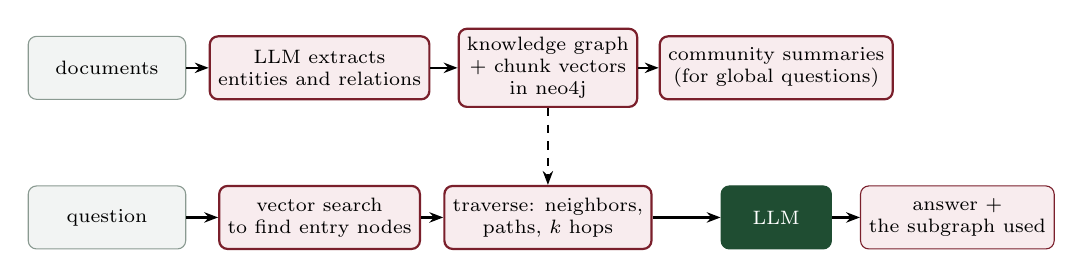
\begin{tikzpicture}[every node/.style={font=\scriptsize, align=center}, >={Stealth[length=5pt]},
      st/.style={draw=bgray, fill=fgray, rounded corners=3pt, minimum height=0.8cm, minimum width=2.0cm, inner sep=3pt},
      hi/.style={draw=burgundy, fill=fburg, thick, rounded corners=3pt, minimum height=0.8cm, minimum width=2.0cm, inner sep=3pt},
      llm/.style={draw=forest, fill=forest, text=white, rounded corners=3pt, minimum height=0.8cm, minimum width=1.4cm}]
    \node[st] (d) at (0,0) {documents};
    \node[hi] (x) at (2.7,0) {LLM extracts\\ entities and relations};
    \node[hi] (g) at (5.6,0) {knowledge graph\\ + chunk vectors\\ in neo4j};
    \node[hi] (s) at (8.5,0) {community summaries\\ (for global questions)};
    \draw[->, thick] (d)--(x); \draw[->, thick] (x)--(g); \draw[->, thick] (g)--(s);
    \node[st] (qq) at (0,-1.9) {question};
    \node[hi] (r1) at (2.7,-1.9) {vector search\\ to find entry nodes};
    \node[hi] (r2) at (5.6,-1.9) {traverse: neighbors,\\ paths, $k$ hops};
    \node[llm] (l) at (8.5,-1.9) {LLM};
    \node[st, draw=burgundy, fill=fburg] (ans) at (10.8,-1.9) {answer +\\ the subgraph used};
    \draw[->, thick] (qq)--(r1); \draw[->, thick] (r1)--(r2); \draw[->, thick] (r2)--(l); \draw[->, thick] (l)--(ans);
    \draw[->, thick, dashed] (g) -- (r2);
  \end{tikzpicture}
  \end{center}
  \vspace{0.2cm}
  \begin{columns}[T]
    \column{0.48\textwidth}
      \small
      \textbf{Workflow}
      \begin{itemize}
        \item build: a model reads each document and proposes entities and relationships; they are merged into a graph with provenance
        \item retrieve: vector search finds a starting point; traversal collects the connected context
        \item answer: the model gets the subgraph and the source chunks
      \end{itemize}
    \column{0.48\textwidth}
      \small
      \textbf{Advantages}
      \begin{itemize}
        \item multi-hop questions become path queries
        \item global questions use precomputed community summaries (Microsoft's GraphRAG, 2024, uses Leiden)
        \item the retrieved subgraph can be shown, so answers can be checked
      \end{itemize}
  \end{columns}
\end{frame}

% ===== SLIDE 38: neo4j AI toolkit =============================================
\begin{frame}[fragile]{neo4j's AI tools}
  \vspace{0.1cm}
  \begin{center}
  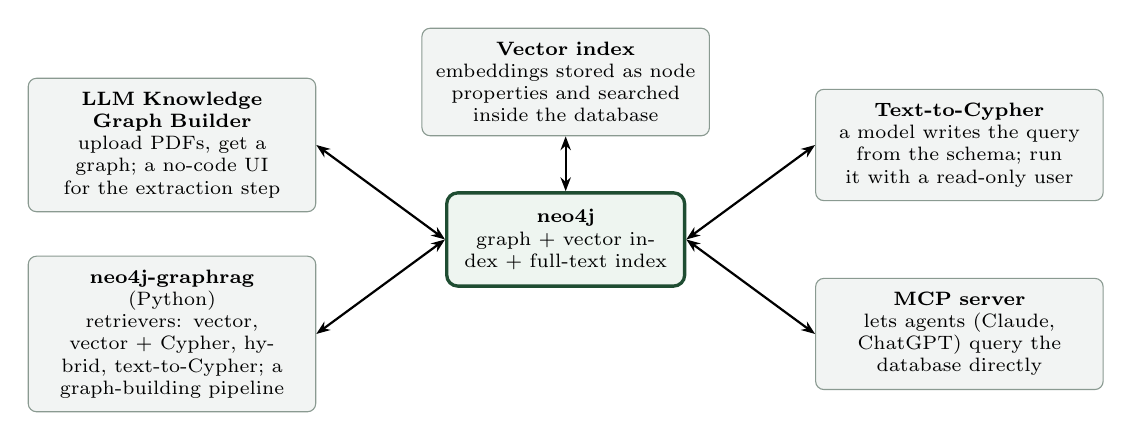
\begin{tikzpicture}[every node/.style={font=\scriptsize, align=center}, >={Stealth[length=5pt]},
      t/.style={draw=bgray, fill=fgray, rounded corners=3pt, text width=3.3cm, inner sep=5pt},
      db/.style={draw=forest, fill=fgreen, very thick, rounded corners=4pt, text width=2.6cm, inner sep=6pt}]
    \node[db] (db) at (0,0) {\textbf{neo4j}\\ graph + vector index + full-text index};
    \node[t] (e) at (0,2.0) {\textbf{Vector index}\\ embeddings stored as node properties and searched inside the database};
    \node[t] (a) at (-5.0,1.2) {\textbf{LLM Knowledge Graph Builder}\\ upload PDFs, get a graph; a no-code UI for the extraction step};
    \node[t] (b) at (-5.0,-1.2) {\textbf{neo4j-graphrag} (Python)\\ retrievers: vector, vector + Cypher, hybrid, text-to-Cypher; a graph-building pipeline};
    \node[t] (c) at (5.0,1.2) {\textbf{Text-to-Cypher}\\ a model writes the query from the schema; run it with a read-only user};
    \node[t] (d) at (5.0,-1.2) {\textbf{MCP server}\\ lets agents (Claude, ChatGPT) query the database directly};
    \draw[<->, thick] (a.east)--(db.west); \draw[<->, thick] (b.east)--(db.west); \draw[<->, thick] (c.west)--(db.east); \draw[<->, thick] (d.west)--(db.east); \draw[<->, thick] (e)--(db);
  \end{tikzpicture}
  \end{center}
  \vspace{0.1cm}
  \small
  \begin{itemize}
    \item With the vector index, chunk embeddings and the knowledge graph are in one database: find by similarity, then expand by relationship, in one query.
    \item \texttt{neo4j-graphrag} is the official Python package for building and querying; text-to-Cypher and the MCP server are how a model asks the database questions on its own.
  \end{itemize}
\end{frame}

% ===== SLIDE 39: when to use ==================================================
\begin{frame}[fragile]{GraphRAG: when it helps and when it does not}
  \vspace{0.3cm}
  \begin{columns}[T]
    \column{0.48\textwidth}
      \begin{tbox}[Use it when]{bgreen}{fgreen}
        \begin{itemize}
          \item questions are relational: who is connected to what, through which steps
          \item the corpus is large and answers draw on many documents at once
          \item answers must be auditable: the subgraph is the evidence
          \item the same entities also need ordinary queries, reports, or dashboards
        \end{itemize}
      \end{tbox}
    \column{0.48\textwidth}
      \begin{tbox}[Plain vector RAG is enough when]{bburg}{fburg}
        \begin{itemize}
          \item a few hundred documents and single-passage questions
          \item the extra cost of extraction (tokens, time, curation) is not justified
        \end{itemize}
      \end{tbox}
      \begin{tbox}[Watch out for]{bgold}{fgold}
        \begin{itemize}
          \item extraction quality: the same relation under five names, entities that split or merge; a fixed schema and identity resolution are required
          \item generated Cypher that is wrong or expensive; use a read-only user and query timeouts
        \end{itemize}
      \end{tbox}
  \end{columns}
\end{frame}

% ===== SLIDE 40: takeaways ====================================================
\begin{frame}[fragile]{Takeaways}
  \vspace{0.4cm}
  \begin{columns}[T]
    \column{0.24\textwidth}
      \begin{tbox}[1 \ Graphs as data]{bgreen}{fgreen}
        A graph database stores relationships next to nodes. Traversals cost what they touch. Use one when questions follow paths or the graph outgrows memory.
      \end{tbox}
    \column{0.24\textwidth}
      \begin{tbox}[2 \ Cypher]{bslate}{fslate}
        Queries are drawn: \texttt{(a)-[:LINE*1..3]-(b)}. The same patterns read and write. Docker gives you a database in two minutes.
      \end{tbox}
    \column{0.24\textwidth}
      \begin{tbox}[{{3 \ GDS}}]{bgold}{fgold}
        Project, run, write back. Degree is local, eigenvector follows density, betweenness finds the bridges. Components show what an outage does.
      \end{tbox}
    \column{0.24\textwidth}
      \begin{tbox}[4 \ Knowledge graphs]{bburg}{fburg}
        Vector search to land, graph to expand, subgraph to check. The hard part moved to building the graph well.
      \end{tbox}
  \end{columns}
  \vspace{0.8cm}
  \centering
  {\Large\bfseries Questions?}\\[6pt]
  \kicker{Docs: neo4j.com/docs/cypher-manual \ $\cdot$ \ neo4j.com/docs/graph-data-science \ $\cdot$ \ neo4j.com/docs/neo4j-graphrag-python}
\end{frame}

% ===== APPENDIX ===============================================================
\appendix
\partslide{A}{Appendix}

% ===== SLIDE A1: cheat sheet ==================================================
\begin{frame}[fragile]{Cypher cheat sheet}
  \vspace{0.1cm}
  \begin{columns}[T]
    \column{0.5\textwidth}
      \begin{code}
// patterns
(n)  (n:Label)  (n:Label {k: v})  (a)-[r:TYPE]->(b)
(a)-[:T*2..4]-(b)        // 2 to 4 hops, any direction
p = (a)-[*]-(b)          // bind a path; nodes(p), length(p)
shortestPath((a)-[:T*]-(b))

// reading
MATCH ... WHERE ... RETURN ... ORDER BY ... LIMIT ...
OPTIONAL MATCH            // left join
WITH x, count(*) AS n     // pipe + aggregate
UNWIND list AS item       // list -> rows
EXISTS { (a)-[:T]->() }   // subquery predicate
      \end{code}
    \column{0.5\textwidth}
      \begin{code}
// writing
CREATE (n:Label {k: v})
MERGE (n:Label {id: 1}) ON CREATE SET ... ON MATCH SET ...
SET n.k = v   REMOVE n.k   DELETE r   DETACH DELETE n

// schema
CREATE CONSTRAINT ... FOR (n:L) REQUIRE n.id IS UNIQUE
CREATE INDEX ... FOR (n:L) ON (n.k)
CREATE VECTOR INDEX ... FOR (n:L) ON (n.emb) OPTIONS {...}

// functions
labels(n) type(r) keys(n) properties(n) elementId(n)
toInteger toFloat toBoolean toString date() point()
size(list) [x IN list | f(x)]  collect() count(DISTINCT x)
      \end{code}
  \end{columns}
\end{frame}

% ===== SLIDE A2: fallback: cypher =============================================
\begin{frame}[fragile]{Fallback: Cypher demo results}
  \vspace{0.1cm}
  \scriptsize
  \begin{columns}[T]
    \column{0.3\textwidth}
      \textbf{Q1 counts}\\[2pt]
      \begin{tabular}{@{}lr@{}}\toprule
        Substation & 140\\ Load & 60\\ Generator & 25\\ \midrule
        LINE & 322\\ SUPPLIES & 60\\ FEEDS & 25\\ \bottomrule
      \end{tabular}\\[8pt]
      \textbf{Q2} Allegheny-01: 69 kV, Allegheny, online\\[8pt]
      \textbf{Q7} shortestPath Allegheny-01 to Pocono-01: 11 hops
    \column{0.36\textwidth}
      \textbf{Q5 generation vs demand (MW)}\\[2pt]
      \begin{tabular}{@{}lrr@{}}\toprule
        region & generation & demand\\ \midrule
        Allegheny & 1846 & 1450\\ Erie & 715 & 728\\ Laurel & 2913 & 629\\ Pocono & 750 & 797\\ Susquehanna & 738 & 639\\ \bottomrule
      \end{tabular}\\[8pt]
      \textbf{Q6 hospitals within 3 lines of a nuclear plant}\\[2pt]
      \begin{tabular}{@{}lll@{}}\toprule
        plant & hospital & via\\ \midrule
        Nuclear-02 & Hospital-01 & Allegheny-24\\
        Nuclear-02 & Hospital-02 & Allegheny-22\\ \bottomrule
      \end{tabular}
    \column{0.32\textwidth}
      \textbf{Q3 / Q4} graph views: Allegheny-01 with its neighbors; two small stars around Nuclear-01 (Laurel) and Nuclear-02 (Allegheny).\\[8pt]
      \textbf{Q8} Allegheny-01, \texttt{inspected} = today's date.
  \end{columns}
\end{frame}

% ===== SLIDE A3: fallback: gds ================================================
\begin{frame}[fragile]{Fallback: GDS demo results}
  \vspace{0.1cm}
  \scriptsize
  \begin{columns}[T]
    \column{0.32\textwidth}
      \textbf{G0} projection: 140 nodes, 644 relationships\\[6pt]
      \textbf{G1 degree}\\[2pt]
      \begin{tabular}{@{}llr@{}}\toprule
        Allegheny-12 & 345 & 8\\ Allegheny-14 & 69 & 8\\ Laurel-02 & 69 & 8\\ Susquehanna-27 & 345 & 8\\ Pocono-08 & 345 & 7\\ Pocono-11 & 138 & 7\\ Pocono-16 & 69 & 7\\ Pocono-23 & 69 & 7\\ \bottomrule
      \end{tabular}
    \column{0.32\textwidth}
      \textbf{G2 eigenvector} (unit-length vector)\\[2pt]
      \begin{tabular}{@{}llr@{}}\toprule
        Pocono-23 & 69 & 0.353\\ Pocono-16 & 69 & 0.331\\ Pocono-08 & 345 & 0.329\\ Pocono-15 & 69 & 0.322\\ Pocono-28 & 69 & 0.283\\ Pocono-05 & 69 & 0.278\\ Pocono-01 & 138 & 0.253\\ Pocono-25 & 69 & 0.240\\ \bottomrule
      \end{tabular}\\[6pt]
      \textbf{G3 betweenness} (raw counts; divide by 9591 to normalize)\\[2pt]
      \begin{tabular}{@{}llr@{}}\toprule
        Susquehanna-27 & 345 & 5171\\ Erie-06 & 345 & 3871\\ Allegheny-12 & 345 & 3600\\ Erie-23 & 345 & 3431\\ Pocono-06 & 345 & 3038\\ \bottomrule
      \end{tabular}
    \column{0.34\textwidth}
      \textbf{G4 components} with Susquehanna-27 offline (139 nodes projected)\\[2pt]
      \begin{tabular}{@{}rlrrr@{}}\toprule
        subs & regions & gen & dem & hosp\\ \midrule
        82 & Alleg., Erie, Laurel & 5474 & 2807 & 4\\
        57 & Pocono, Susq. & 1488 & 1436 & 2\\ \bottomrule
      \end{tabular}\\[8pt]
      \textbf{G5} \texttt{betweenness.write}: 140 properties written; top five as in G3.\\[8pt]
      Figures for G1--G4 are on slides 30--33.
  \end{columns}
\end{frame}

\end{document}
